\section{Полная проверка выбора маршрутизатора при дисбалансе}
Предыдущие сравнения сохраняются как промежуточные контроли.
Выводы о полном наборе методов далее основаны на расширенной семье:
20 вместо 30 повторений, все восемь обучаемых методов вместо двух
в контроле обогащения и девять вместо четырёх кандидатов selector.
Значимость в прежней узкой семье не переносится автоматически
на новый протокол и его общую поправку.
\subsection{От профиля решений к проверяемой гипотезе}
Разные способы обучения могут иметь близкую accuracy, выбирая разные
запросы. Если один метод одновременно чаще спасает ошибки и чаще
портит правильные ответы, итоговая разность может компенсироваться.
Это мотивирует гипотезу: изменение состава парной разметки способно
неодинаково повлиять на методы и изменить их сравнительное качество.
Она проверяется взаимодействием \emph{метод $\times$ состав},
а не только эффектом коррекции одного оценивателя.

Используется полный набор восьми обучаемых способов
из таблицы~\ref{tab:all_methods}, confidence и случайное ранжирование.
К четырём исходным экспертам относятся TF--IDF, BERT-tiny, frozen
и fine-tuned MiniLM. Добавлены три ранее обученные TF--IDF-модели
с 1/3/10 размеченными примерами каждого из 77 классов; их словарь
фиксирован по исходной expert-train части. Проверены все 21 прежняя
пара, а не выбранные по новому test-эффекту примеры.
Эксперты не переобучаются. Направления low-label пар не всегда
соответствуют росту стоимости; флаг порядка стоимости и полные
параметры сохранены в \texttt{code/data/imbalance\_manifest.json}.

\subsection{Факторная сетка и метрики}
Fit содержит 200, 500 или 1\,000 извлечений с возвращением;
20 seeds и квоты 10/20/40\%. Семь составов --- natural,
rescue с множителем 2 или 8, harm с множителем 2 или 8,
discordant с множителем 8 и neutral с множителем 8.
Четыре сильных обогащения дополнительно проверены с IPW
у всех восьми методов на тех же fit-строках.
Всего получены 1\,260 условий pair/seed/size и 110\,880 выбранных
роутеров после 443\,520 кандидатов регуляризации.
Признаки, сетка регуляризации, естественный tuning-dev размера $n/2$
и отдельный selector-dev500 общие. Для каждого варианта состава
selector выбирает из восьми обучаемых методов и confidence.

Помимо accuracy и gain MSE измеряются precision, recall и F1
спасений, частота вредных замен, доля найденных вредных исходов
и доля предотвращённого вреда. При $R$ спасениях, $H$ вредных
заменах, $k$ вызовах и $N_+$ доступных спасениях:
\begin{equation}
\operatorname{precision}_{+}=\frac{R}{k},\qquad
\operatorname{recall}_{+}=\frac{R}{N_+},\qquad
F1_+=\frac{2R}{k+N_+},\qquad
\operatorname{harm\ rate}=\frac{H}{k}.
\end{equation}
При фиксированной паре и квоте три метрики спасений связаны
одним числом $R$, поэтому не считаются независимыми подтверждениями.
Accuracy определяется $R-H$, что допускает разные профили.
Recall при отсутствии соответствующего события не определён,
а не приравнен искусственно к нулю.

\subsection{Общая статистическая семья}
Основная область --- все 21 пары, fit1000, квота20\%, official test.
Проверены 5\,691 контраст: 2\,268 простых попарных accuracy-различий
в natural/rescue8/harm8, 1\,512 взаимодействий с составом,
1\,512 различий natural-профилей, 336 IPW--raw и 63
selector--confidence. Использованы 2\,000 crossed paired bootstrap
повторов с точным пересчётом квоты и одной общей max-$|t|$ поправкой.
Семья и сетка зафиксированы до запуска; меньшие объёмы, слабое
обогащение, neutral/discordant, остальные квоты и clean-test
сохраняются как описательные проверки устойчивости.

После общей поправки в natural обнаружено 0 из 756 попарных accuracy-различий (0 из 441 между семью gain-оценивателями). При этом в 0 сравнениях различим профиль спасений/вреда без обнаруженного accuracy-различия; это не доказательство эквивалентности accuracy.

Взаимодействие метода и состава поддержано в 56 из 1512 контрастов, в том числе в 0 из 882 между семью gain-оценивателями. Оно встречается в 4 из 21 пары (gain-only: 0). Эти пары зависимы и не являются независимыми задачами.

Поддержанных смен знака преимущества, при которых оба простых одновременных интервала лежат по разные стороны нуля, получено 0 (gain-only: 0). Значимое взаимодействие само по себе не требует смены победителя и не заменяет проверку простых эффектов.

Из 336 изменений отдельных методов от natural при rescue8/harm8 0 являются улучшениями и 28 --- ухудшениями после той же общей поправки. Эти проверки уже входят в семью как взаимодействия с неизменным confidence.


\begin{table}[htbp]\centering\small
\caption{Средняя accuracy, \%, по 20 обучениям при fit1000 и квоте20\%
для двух исходных пар, полный набор девяти правил. Это иллюстративные
средние; все SD, интервалы и остальные пары опубликованы отдельно.}
\begin{tabular}{lrrrrrr}
\toprule
 & \multicolumn{3}{c}{TF--IDF $\to$ BERT-tiny} & \multicolumn{3}{c}{TF--IDF $\to$ MiniLM} \\
Метод & Natural & Rescue8 & Harm8 & Natural & Rescue8 & Harm8 \\
\midrule
Weak-error & 87.87 & 87.89 & 87.67 & 91.26 & 91.30 & 91.25 \\
Direct & 87.61 & 88.22 & 86.38 & 91.44 & 91.57 & 86.56 \\
Marginal & 87.58 & 87.92 & 86.41 & 91.36 & 91.31 & 86.50 \\
Events & 87.50 & 87.93 & 86.40 & 91.45 & 91.35 & 86.50 \\
Ternary & 87.37 & 87.95 & 86.43 & 91.46 & 91.33 & 86.61 \\
Joint & 87.42 & 87.93 & 86.43 & 91.43 & 91.32 & 86.61 \\
Hurdle & 87.82 & 87.92 & 86.43 & 91.34 & 91.38 & 86.61 \\
Soft-gain & 87.59 & 88.04 & 86.38 & 91.37 & 91.33 & 86.52 \\
Confidence & 87.24 & 87.24 & 87.24 & 90.68 & 90.68 & 90.68 \\
\bottomrule
\end{tabular}

\end{table}

\begin{figure}[htbp]\centering
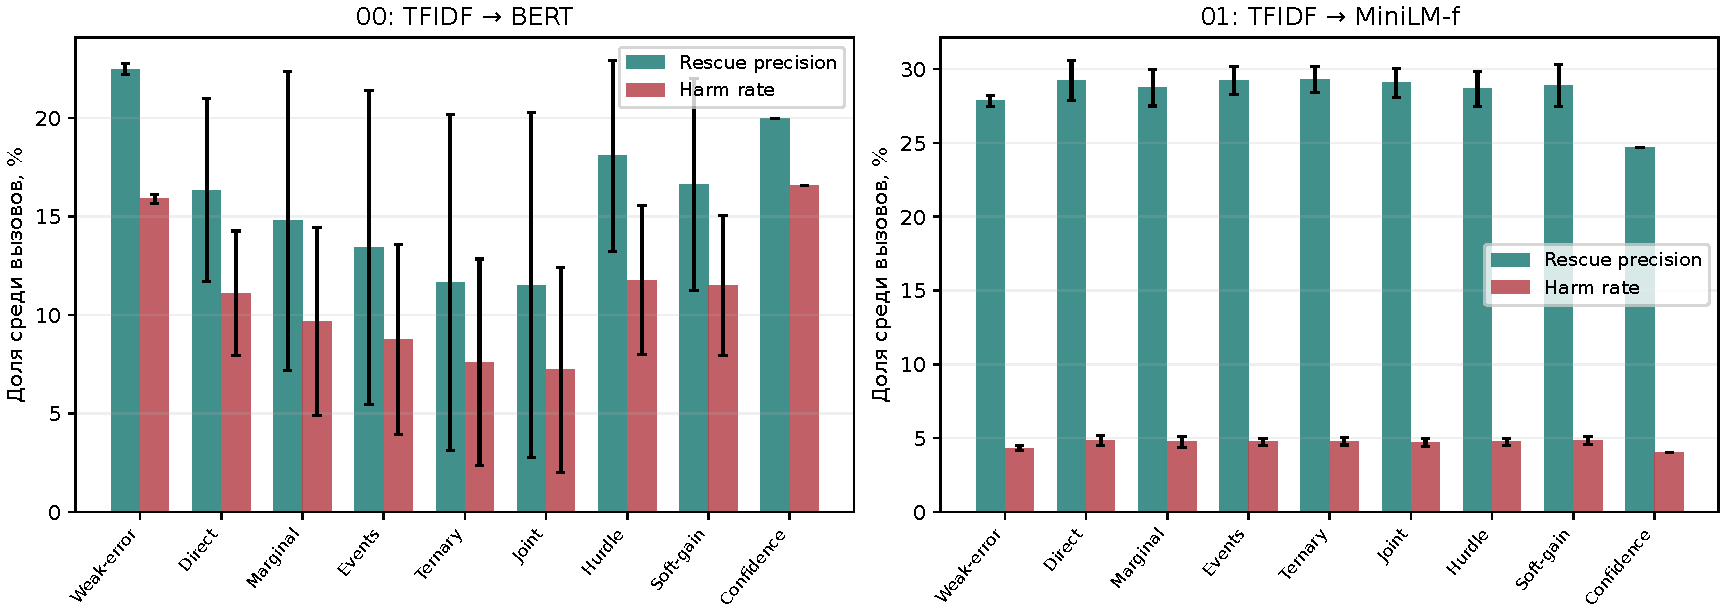
\includegraphics[width=\linewidth]{figures/imbalance_natural_profiles.pdf}
\caption{Natural-профили всех правил на двух исходных парах:
доли спасений и вреда среди эскалаций, средние и SD по 20 seeds.
Нужно сравнивать оба компонента, а не только итоговую accuracy.}
\end{figure}

\begin{figure}[htbp]\centering
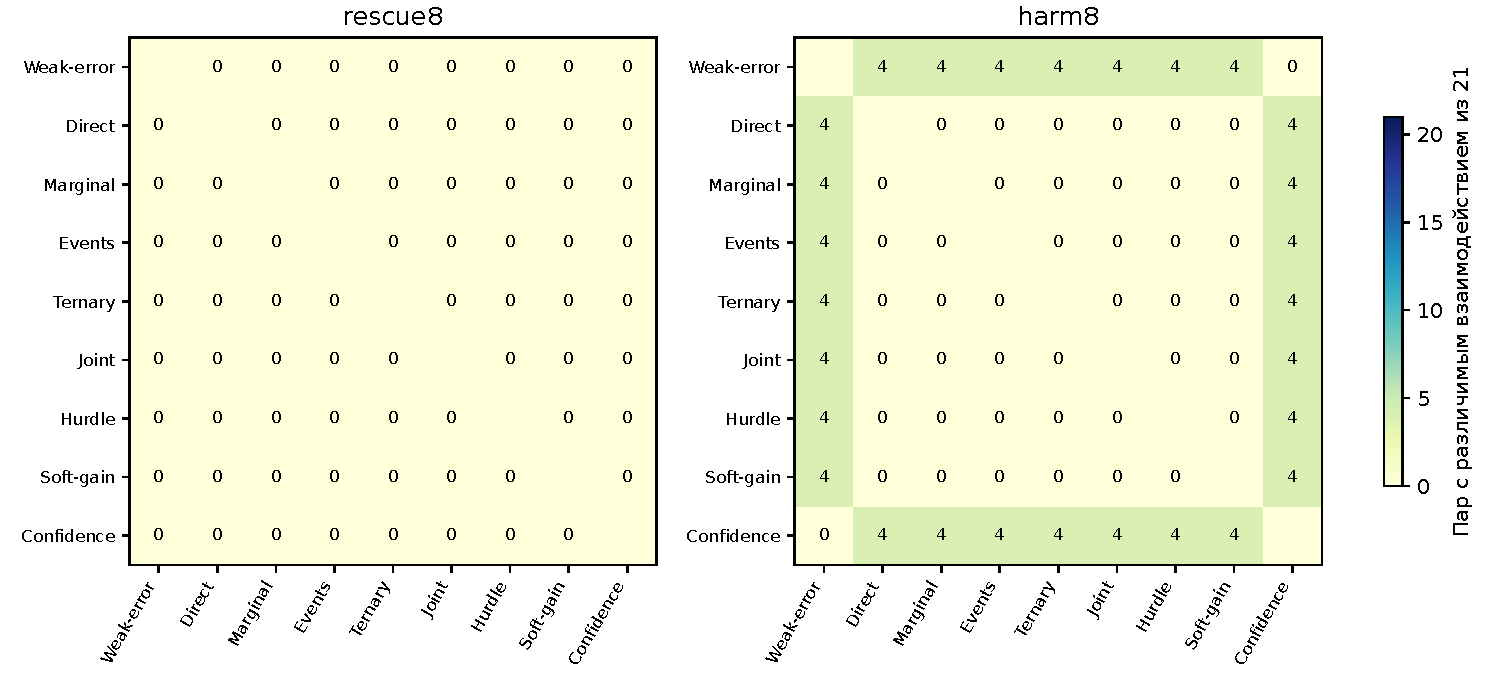
\includegraphics[width=\linewidth]{figures/imbalance_interaction_counts.pdf}
\caption{Число пар из 21 с различимым взаимодействием каждой пары
методов и состава после общей поправки. Это зависимые конфигурации
одного датасета; семь gain-методов отделяются от weak-error/confidence.}
\end{figure}

\subsection{Интерпретация и воспроизводимость}
Гипотеза о чувствительности методов проверяется на фактических
взаимодействиях. Для выбора метода важно дополнительно отличать
изменение величины преимущества от надёжной смены предпочтительности,
а улучшение от natural --- от неодинакового ухудшения методов.
Коррекция служит контролем механизма смещения обучающей цели,
но не заменяет основную задачу выбора маршрутизатора.

Все модели, ID извлечений, weights и scores сохраняются локально;
опубликованы полный per-seed результат, сводки, частоты выбора,
regret и все статистические контрасты в
\texttt{paper/imbalance\_results/}. Запуск:
\texttt{code/imbalance\_study.py}, аудит:
\texttt{code/audit\_imbalance.py}, статистика:
\texttt{code/imbalance\_statistics.py}, отчёт:
\texttt{code/analyze\_imbalance.py}. Контроль повторно использует
ранее изученный BANKING77 test. Он позволяет изучать чувствительность
и локальный выбор, но не устанавливает переносимость рекомендации
на независимые задачи.
